\documentclass{assignment}
\usepackage[utf8]{inputenc}
\usepackage[T1]{fontenc}
\usepackage{hyperref}
\usepackage{listings}

\lstset{
	inputencoding=utf8,
	literate=
	{á}{{\'a}}1
	{é}{{\'e}}1
	{í}{{\'i}}1
	{ó}{{\'o}}1
	{ú}{{\'u}}1
	{Á}{{\'A}}1
	{É}{{\'E}}1
	{Í}{{\'I}}1
	{Ó}{{\'O}}1
	{Ú}{{\'U}}1
	{ñ}{{\~n}}1
	{Ñ}{{\~N}}1
}


\lstdefinelanguage{Pseudocodigo}{
	morekeywords={
		SI, ENTONCES, SINO, FIN, MIENTRAS, HACER, PARA, DESDE, HASTA,
		FUNCIÓN, PROCEDIMIENTO, CLASE, CONSTRUCTOR, ATRIBUTOS,
		RETORNAR, ALGORITMO, CONSTANTE, NUEVO, Y, O, NO, CADA, EN
	},
	sensitive=false,
	morecomment=[l]{//},
	morestring=[b]",
}

\lstset{
	language=Pseudocodigo,
	basicstyle=\ttfamily\small,
	keywordstyle=\color{blue}\bfseries,
	commentstyle=\color{gray}\itshape,
	stringstyle=\color{orange},
	numbers=left,
	numberstyle=\tiny\color{gray},
	stepnumber=1,
	breaklines=true,
	frame=single,
	tabsize=4,
	showstringspaces=false,
}
\begin{document}
	
	\assignmentTitle{Claudio Iván Esparza Castañeda}{Luis Alberto Balam Guzmán}{./Logo.png}{Maestría en Sistemas Embebidos}{Programación y Procesamiento de Datos}{3A. Práctica de manejo de datos en Python}
	
	\section*{Objetivo}
	Más allá de las funciones incluidas en el estándar de Python, la amplia comunidad comenzó a implementar funciones más complejas que agrupan múltiples funciones orientadas a tópicos específicos. La idea es que no se tenga que reinventar la rueda cada vez. Con este espíritu es que se crearon módulos (propiamente el equivalente de las bibliotecas o librería de otros lenguajes) como pandas, el cual tiene funciones para manipular los arreglos mixtos como dataframe, yendo más allá de los datos numéricos, permite interpretar otras utilidades como el tipo fecha, o las múltiples combinaciones propias del tipo texto. Otra de gran utilidad es Matplotlib, que contiene múltiples representaciones gráficas para los datos obtenidos con otros módulos.\\
	La popularidad de Pandas en combinación de Matplotlib de manera reciente viene de su uso en análisis de datos, de la inteligencia artificial, entre otros campos. Las aplicaciones, claro, son infinitas y corresponde a uno plantearse la manera en que quisiera realizar estas tareas.\\
	Se retoma el reciclaje de funciones, sin ninguna adición.\\
	Combinando los conocimientos usados en las pácticas anteriores, se combina para tener clases, listas iterables, y ahora el uso de pandas y Matplotlib para tener dataframes y su representación gráfica.\\
	Este programa involucra el uso de un menú para el control del flujo. Se cuenta con validaciones para los distintos tipos de datos que se emplean en el programa, y se cuenta con una Clase "Clima" con métodos para cada etapa opción del menú.
		\section*{Capturas de ejecución}
	\begin{figure}[htbp]
		\centering
		
\includegraphics[width=0.6\textwidth]{Figuras/1}
		\caption{Validación de archivo de entrada no encontrado.}
		\label{fig:1}
	\end{figure}
	\begin{figure}[htbp]
		\centering
		
\includegraphics[width=0.5\textwidth]{Figuras/2}
		\caption{Opción 2 no realizada por falta de datos cargados.}
		\label{fig:2}
	\end{figure}
	\begin{figure}[htbp]
		\centering
		
\includegraphics[width=0.5\textwidth]{Figuras/3}
		\caption{Opción 3 no realizada por falta de datos cargados.}
		\label{fig:3}
	\end{figure}
	\begin{figure}[htbp]
		\centering
		
\includegraphics[width=0.5\textwidth]{Figuras/4}
		\caption{Opción 4 no realizada por falta de datos cargados.}
		\label{fig:4}
	\end{figure}
	\begin{figure}[htbp]
		\centering
		
\includegraphics[width=0.5\textwidth]{Figuras/5}
		\caption{Opción 5 no realizada por falta de datos cargados.}
		\label{fig:5}
	\end{figure}
	
	\begin{figure}[htbp]
		\centering
		
\includegraphics[width=0.5\textwidth]{Figuras/6}
		\caption{Opción 6 no realizada por falta de datos cargados.}
		\label{fig:6}
	\end{figure}
	\begin{figure}[htbp]
		\centering
		
\includegraphics[width=0.5\textwidth]{Figuras/7}
		\caption{Salida correcta del programa}
		\label{fig:7}
	\end{figure}
	\begin{figure}[htbp]
		\centering
		
\includegraphics[width=0.5\textwidth]{Figuras/8}
		\caption{Carga correcta de datos.}
		\label{fig:8}
	\end{figure}
	\begin{figure}[htbp]
		\centering
		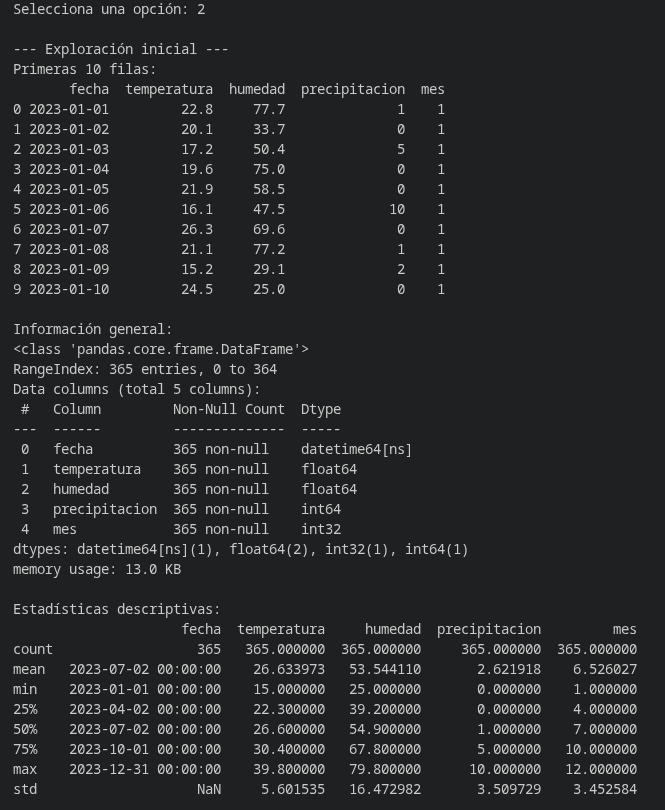
\includegraphics[width=0.55\textwidth]{Figuras/9}
		\caption{Exploración inicial.}
		\label{fig:9}
	\end{figure}
	\begin{figure}[htbp]
		\centering
		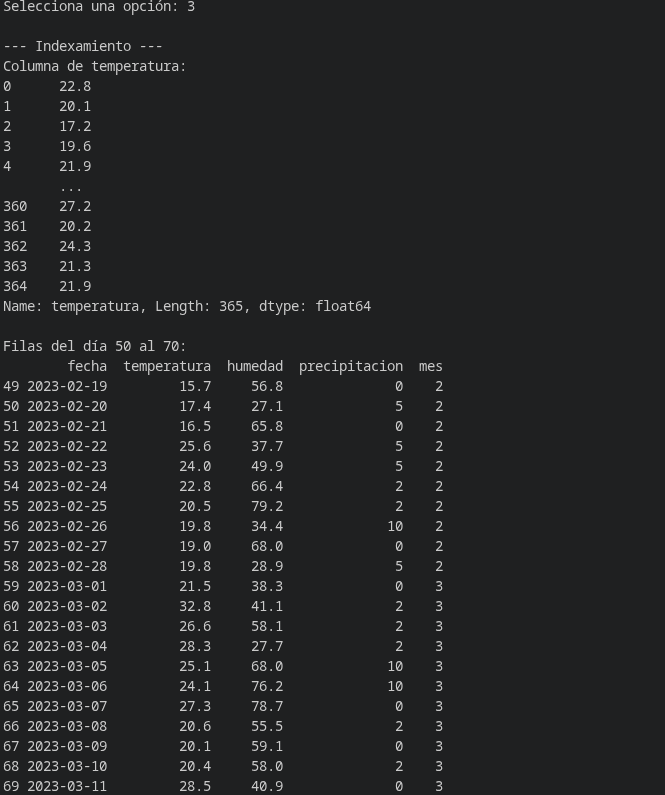
\includegraphics[width=0.55\textwidth]{Figuras/10}
		\caption{Indexamiento.}
		\label{fig:10}
	\end{figure}
	\begin{figure}[htbp]
		\centering
		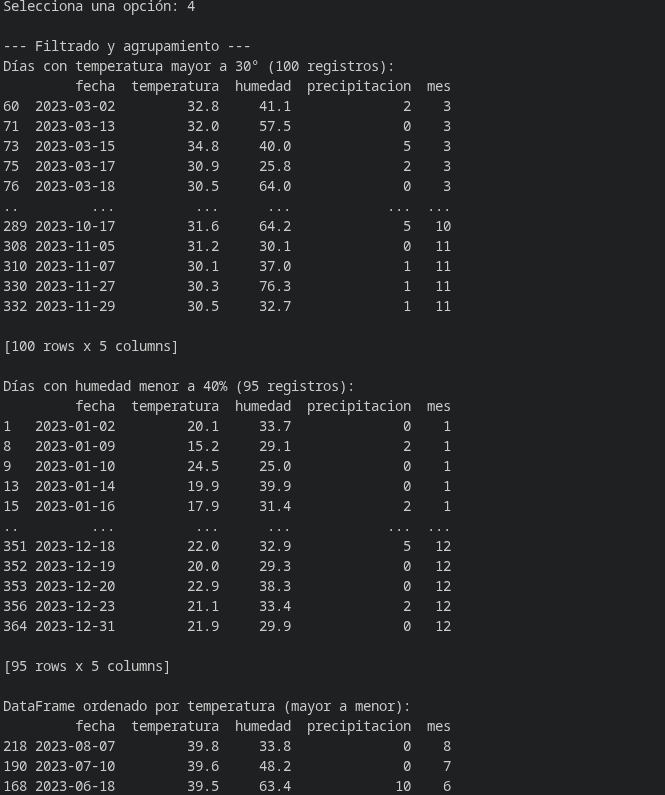
\includegraphics[width=0.55\textwidth]{Figuras/11}
		\caption{Filtrado y agrupamiento.}
		\label{fig:11}
	\end{figure}
	\begin{figure}[htbp]
		\centering
		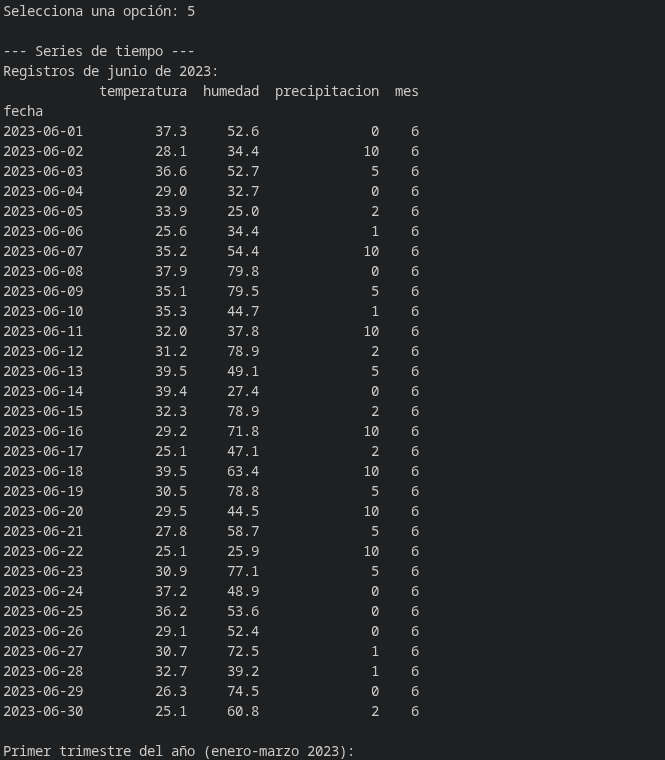
\includegraphics[width=0.55\textwidth]{Figuras/12}
		\caption{Series de tiempo.}
		\label{fig:12}
	\end{figure}
	\begin{figure}[htbp]
		\centering
		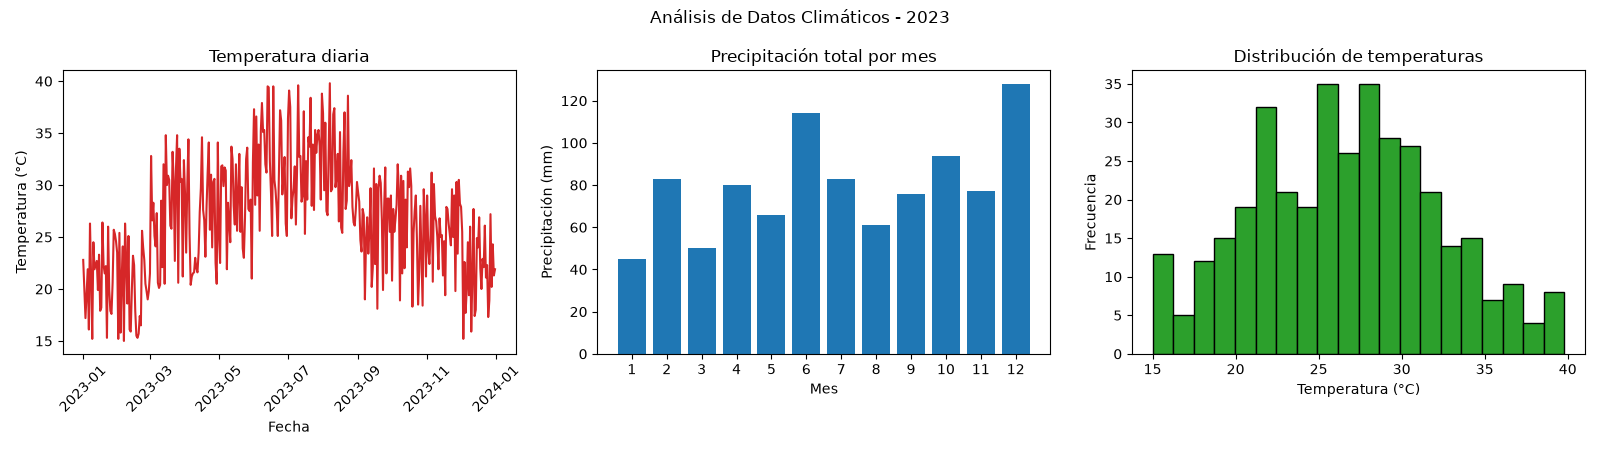
\includegraphics[width=\textwidth]{Figuras/13}
		\caption{Gráficas.}
		\label{fig:13}
	\end{figure}
		\section*{Pseudocódigo}
	Ya desde prácticas anteriores PSeInt estaba rebasado para plasmar estos algoritmos más complejos, aquí traté de expresarlo en lenguaje natural. Por la simpleza de python, mucho fue traducir de inglés a español.
	\subsection*{Inicialización}
	\begin{lstlisting}[caption={Inicialización}, label={lst:inicio}]
		CONSTANTE ARCHIVO_CSV <- "clima_2023.csv"
		CONSTANTE COLUMNAS_REQUERIDAS <- {"fecha", "temperatura", "humedad", "precipitacion"}
		PROCEDIMIENTO Menu()
			IMPRIMIR "===== MENÚ PRINCIPAL ====="
			IMPRIMIR "1. Cargar datos"
			IMPRIMIR "2. Exploración inicial"
			IMPRIMIR "3. Indexamiento"
			IMPRIMIR "4. Filtrado y agrupamiento"
			IMPRIMIR "5. Series de tiempo"
			IMPRIMIR "6. Gráficas"
			IMPRIMIR "7. Salir"
		FIN PROCEDIMIENTO
	\end{lstlisting}
	\subsection*{Clase Clima}
		\begin{lstlisting}[caption={Clase Clima}, label={lst:clima}]
		CLASE ClimaPandas
			ATRIBUTOS
				df : DataFrame
			CONSTRUCTOR ClimaPandas()
				df <- NULO
			FIN CONSTRUCTOR
			FUNCIÓN HayDatos(): Booleano
				SI df = NULO ENTONCES
					IMPRIMIR "Primero debes cargar los datos (opción 1)."
				RETORNAR FALSO
				FIN SI
				RETORNAR VERDADERO
			FIN FUNCIÓN
			PROCEDIMIENTO AsegurarIndiceFecha()
				SI el índice de df NO es de tipo fecha ENTONCES
					df <- EstablecerIndice(df, "fecha")
					df <- OrdenarPorIndice(df)
				FIN SI
			FIN PROCEDIMIENTO
			PROCEDIMIENTO CargarDatos()
				IMPRIMIR "--- Cargar datos ---"
				INTENTAR
					datos <- LeerCSV(ARCHIVO_CSV)
				CAPTURAR ArchivoNoEncontrado
					IMPRIMIR "No se encontró el archivo '", ARCHIVO_CSV, "'."
					RETORNAR
				CAPTURAR ArchivoVacio
					IMPRIMIR "El archivo '", ARCHIVO_CSV, "' está vacío."
					RETORNAR
				FIN INTENTAR
				SI NO ColumnasRequeridasPresentes(datos, COLUMNAS_REQUERIDAS) ENTONCES
					IMPRIMIR "El archivo no tiene las columnas esperadas: ", COLUMNAS_REQUERIDAS
					IMPRIMIR "Columnas encontradas: ", ColumnasDe(datos)
					RETORNAR
				FIN SI
				datos["fecha"] <- ConvertirADatetime(datos["fecha"])
				datos["mes"] <- ExtraerMes(datos["fecha"])
				df <- datos
				IMPRIMIR "Datos cargados correctamente: ", CantidadFilas(df), " registros."
			FIN PROCEDIMIENTO
			PROCEDIMIENTO Exploracion()
				IMPRIMIR "--- Exploración inicial ---"
				SI NO HayDatos() ENTONCES
					RETORNAR
				FIN SI
				IMPRIMIR "Primeras 10 filas:"
				IMPRIMIR PrimerasFilas(df, 10)
				IMPRIMIR "Información general:"
				IMPRIMIR InformacionGeneral(df)
				IMPRIMIR "Estadísticas descriptivas:"
				IMPRIMIR EstadisticasDescriptivas(df) // media, min, max, cuartiles, etc.
			FIN PROCEDIMIENTO
			PROCEDIMIENTO Indexamiento()
				IMPRIMIR "--- Indexamiento ---"
				SI NO HayDatos() ENTONCES
					RETORNAR
				FIN SI
				IMPRIMIR "Columna de temperatura:"
				IMPRIMIR df["temperatura"]
				IMPRIMIR "Filas del día 50 al 70:"
				IMPRIMIR FilasPorPosicion(df, DESDE 49 HASTA 69)   // día n = posición n-1
				IMPRIMIR "Temperatura y humedad de los primeros 100 registros:"
				IMPRIMIR PrimerasFilas(df[["temperatura", "humedad"]], 100)
				IMPRIMIR "Temperatura del día 120: ", FilaPorPosicion(df, 119)["temperatura"]
				IMPRIMIR "Humedad del día 200: ", FilaPorPosicion(df, 199)["humedad"]
			FIN PROCEDIMIENTO
			PROCEDIMIENTO FiltradoAgrupamiento()
				IMPRIMIR "--- Filtrado y agrupamiento ---"
				SI NO HayDatos() ENTONCES
					RETORNAR
				FIN SI
				calidos <- Filtrar(df, temperatura > 30)
				IMPRIMIR "Días con temperatura mayor a 30 (", CantidadFilas(calidos), " registros):"
				IMPRIMIR calidos
				secos <- Filtrar(df, humedad < 40)
				IMPRIMIR "Días con humedad menor a 40% (", CantidadFilas(secos), " registros):"
				IMPRIMIR secos
				ordenado <- OrdenarPor(df, "temperatura", DESCENDENTE)
				IMPRIMIR "DataFrame ordenado por temperatura (mayor a menor):"
				IMPRIMIR ordenado
				agrupado <- AgruparPor(df, "mes") CON
				temperatura_promedio <- Media(temperatura)
				humedad_promedio     <- Media(humedad)
				precipitacion_total  <- Suma(precipitacion)
				IMPRIMIR "Agrupamiento por mes:"
				IMPRIMIR agrupado
			FIN PROCEDIMIENTO
			PROCEDIMIENTO SeriesTiempo()
				IMPRIMIR "--- Series de tiempo ---"
				SI NO HayDatos() ENTONCES
					RETORNAR
				FIN SI
				AsegurarIndiceFecha()
				IMPRIMIR "Registros de junio de 2023:"
				IMPRIMIR df[fecha PERTENECE A "2023-06"]		
				IMPRIMIR "Primer trimestre del año (enero-marzo 2023):"
				IMPRIMIR df[fecha ENTRE "2023-01" Y "2023-03"]		
				promedio_semanal <- PromedioPorSemana(df["temperatura"])   // resample semanal
				IMPRIMIR "Promedio semanal de temperatura:"
				IMPRIMIR promedio_semanal
			FIN PROCEDIMIENTO
			PROCEDIMIENTO Graficas()
				IMPRIMIR "--- Gráficas ---"
				SI NO HayDatos() ENTONCES
					RETORNAR
				FIN SI
				AsegurarIndiceFecha()
				CREAR figura CON 1 fila Y 3 columnas DE subgráficas: panel_linea, panel_barras, panel_hist
				TituloGeneral(figura, "Análisis de Datos Climáticos - 2023")
				DibujarLinea(panel_linea, eje_x <- df.indice, eje_y <- df["temperatura"], color <- ROJO)
				Titulo(panel_linea, "Temperatura diaria")
				EtiquetaEjeX(panel_linea, "Fecha")
				EtiquetaEjeY(panel_linea, "Temperatura (C)")
				RotarEtiquetasEjeX(panel_linea, 45)
				precipitacion_mensual <- AgruparPor(df, "mes") Y Sumar(precipitacion)
				DibujarBarras(panel_barras, eje_x <- precipitacion_mensual.meses,
				eje_y <- precipitacion_mensual.valores, color <- AZUL)
				Titulo(panel_barras, "Precipitación total por mes")
				EtiquetaEjeX(panel_barras, "Mes")
				EtiquetaEjeY(panel_barras, "Precipitación (mm)")
				DibujarHistograma(panel_hist, datos <- df["temperatura"], num_barras <- 20, color <- VERDE)
				Titulo(panel_hist, "Distribución de temperaturas")
				EtiquetaEjeX(panel_hist, "Temperatura (C)")
				EtiquetaEjeY(panel_hist, "Frecuencia")
				MostrarFigura(figura)
			FIN PROCEDIMIENTO
		FIN CLASE
	\end{lstlisting}
	\subsection*{Algoritmo principal}
	\begin{lstlisting}[caption={Algoritmo principal}, label={lst:principal}]
		ALGORITMO Principal
			opcion <- 0
			clima <- NUEVO ClimaPandas()
			Menu()
			MIENTRAS opcion <> 7 HACER
				opcion <- PedirEntero("Selecciona una opción: ")
				SI opcion = 1 ENTONCES		
					clima.CargarDatos()
				SINO SI opcion = 2 ENTONCES
					clima.Exploracion()
				SINO SI opcion = 3 ENTONCES
					clima.Indexamiento()
				SINO SI opcion = 4 ENTONCES
					clima.FiltradoAgrupamiento()
				SINO SI opcion = 5 ENTONCES
					clima.SeriesTiempo()
				SINO SI opcion = 6 ENTONCES
					clima.Graficas()
				SINO SI opcion <> 7 ENTONCES
					IMPRIMIR "Opción no válida"
				FIN SI
				SI opcion <> 7 ENTONCES
					Menu()
				FIN SI
			FIN MIENTRAS
			IMPRIMIR "Finalizando el programa..."
		FIN ALGORITMO
	\end{lstlisting}
	
	\section*{Conclusiones}
	La reusabilidad de funciones usadas en tareas anteriores contribuye a tener código reusable en todos los niveles.\\
	Junto con NumPy, pandas y Matplotlib se han ganado un lugar entre los módulos más usados para tareas que manejan muchísimos datos en Python. Sus aplicaciones abarcan múltiples campos.
	La carpeta en el repositorio de este proyecto es: \href{https://github.com/clivan/Programacion_y_Procesamiento_de_Datos_Infotec/3A}{Programación y procesamiento de Datos}.	
\end{document}
